\section{My implementation of the L* and NL*}
During this semester, I've implemeted the two algorithms to better understand them and at the end to be able to compare their performances.

\subsection{About the Teacher}
In this report I have barely explained what a \textit{Teacher} is. As said in the Introduction, a \textit{Teacher} is an entity knowing the language and answering to membership and equivalence quieries. It is easy to see how a membership query can be answered: if the \textit{Teacher} knows the language, it can only submit the received word to the langauge and check if the word is in it.

However it is less evident how the \textit{Teacher} should verify if a conjecture is valid or if not to send the counter-example.
\begin{definition}
  The \textit{Teacher} providing every time a counter-exemple of shortest length is called \textit{Minimal Adequate Teacher}.
\end{definition}

From this moment on let's suppose that the \textit{Teacher} is the \textit{Minimal Adequate Teacher} and that the language is represent by the \textit{Automaton} \automaton{}.

When the \textit{Learner} sends the conjecture $\mathcal{A}'$, the \textit{Teacher} has to perform the simmetrical difference of $L(\mathcal{A}) \Delta L(\mathcal{A'})$ to find the counter-example of shortest length. This operation can be made in the following way :

\begin{algorithm}
  \caption{Shortest counter-example in $L(\mathcal{A}) \Delta L(\mathcal{A'})$}
  $A_1 \gets \mathcal{A} \cap \bar{\mathcal{A'}}$\;
  $A_2 \gets \mathcal{A'} \cap \bar{\mathcal{A}}$\;
  $w_1 \gets \text{ the shortest word accepted by } A_1$\;
  $w_2 \gets \text{ the shortest word accepted by } A_2$\;
  \Return shortest($w_1, w_2$)\;
\end{algorithm}

Note that the complementation of a \textit{Automaton} \automaton{} works if \automaton{} is determinized (one of the most expensive operation over \textit{Automata}) and the final states become non-final and vice-versa. The intersection is done thanks to the cartesian product of the two \textit{Automata} and the shortest word accepted by an automaton can be done with a \textit{BFS} algorithm over the automaton.

In this way we are guaranteed that the \textit{Teacher} is the \textit{Minimal Adequate Teacher} but we can also see that it is preferable to have a \textit{Learner} which send more membership queries instead of equivalence queries to decomplexify the learning phase.

\subsection{About the HTML implementation}

I've decided to use TypeScript as programming language to be able to easily display the execution of these algorithms thanks to a dedicated HTML page.

The page is available at \url{https://fissored.github.io/TER-M1-S2/} and allows to choose both to run the \textit{L*} and the \textit{NL*} algorithms. Some preload Theachers have been upload to let the uses test immediatly them but it is also possible to enter a choosen regular expression to build the Teacher and pass it to the Learner.

The regular expression should be encoded with the following grammar :
\[ R = symbol \; | \; R + R \; | \; RR \; | \;R^* \; | \;(R) \]
where symbol can be every alpha-numeric character. The empty string $\varepsilon$ is encoded with the $\$$ symbol.

\begin{example}
  \[(a + b)+\$+ab^*+(ab)^*\] indicates the language containg $\{\varepsilon,a, b,  ab, abb, abbb\dots, ab, abab, ababab\dots\}$.
\end{example}

Once the Teacher created, the user can run step by step or the entire algorithm and every phase of the execution will be displayed. The \textit{Message} section contains information about the \textit{closedness} and the \textit{consistence} of the $O.T$. Once these two properties are satisfied, the automaton corresponding to the conjecture is displayed (thanks the \textit{d3-graphviz.js} library).

You can see test word membership with the buttons next to the automaton.

If a counter-exemple is provided then it is written in the \textit{Message} section otherwise the automaton has been approved and the algorithm can stop.

The history of the operations made by the \textit{Learner} is saved in memory and can be re-taken with the arrows on the side of the screen.

\subsection{Script for testing}
Once compiled in JavaScript, the source files which doesn't need a browser to work, can be run in terminal thanks to the NodeJs environment. \\
This has allowed me to create some files to test the performances of the two algorithms in term of how many interaction are performed between the \textit{Learner} and \textit{Teacher}, the number of state of the final conjectures of the two algorithms and so on. \\
All of this statistics are written in a CSV file and the transformed into plots with the \textit{mathplotlib} library of Python.\\
The test of comparaison aims to provide \textit{Teachers} to the two \textit{Learners} and then to find the limits of them. As said in \cref{sec:RFSA}, the number of state of a canical \textit{RFSA} may be equal of exponentially smaller then a \textit{mDFA}. So it is interesting to compare \textit{L*} and \textit{NL*} on languages which touches the two bounds of the \textit{RFSA}.


\subsubsection{Size(RFSA) is exponentially smaller then Size(mDFA)}
Languages recognizing by the regular expression $U = regex((a+b)^*a(a+b)^n)$ for a fixed $n$ is knwon to build automaton whose number of states increse exponentially every time we increase the value of $n$. However $U$ can be represented by a \textit{mNFA} whose number of state is equal to $n+1$ and each of this states represent a prime residual. So we can intuitively understand that $U$ can be also represented by a canonical \textit{RFSA} which has the same number of the \textit{NFA}.

\begin{figure}[!htb]
  \centering
  \begin{subfigure}[b]{0.3\textwidth}
    \includegraphics[width=\textwidth]{../statistics/plots/wrostDFA/State nb in A.png}
    \caption{Comparing State Number}
    \label{fig:StateWrostDFACompare}
  \end{subfigure}
  \begin{subfigure}[b]{0.3\textwidth}
    \includegraphics[width=\textwidth]{../statistics/plots/wrostDFA/Equivalence queries.png}
    \caption{Equivalence queries Number}
    \label{fig:EquivWrostDFACompare}
  \end{subfigure}
  \begin{subfigure}[b]{0.3\textwidth}
    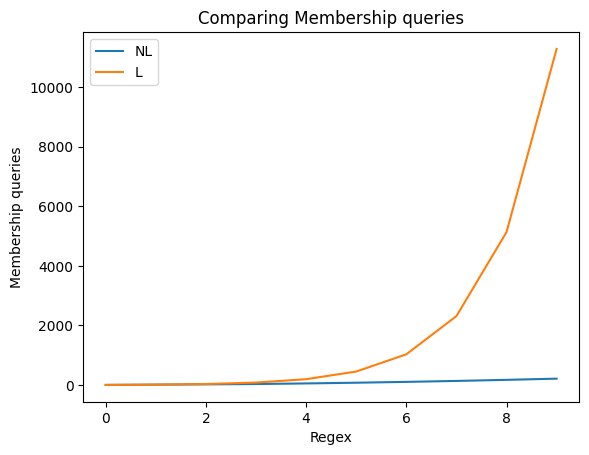
\includegraphics[width=\textwidth]{../statistics/plots/wrostDFA/Membership queries.png}
    \caption{Membership queries Number}
    \label{fig:MemberWrostDFACompare}
  \end{subfigure}
  \begin{subfigure}[b]{0.3\textwidth}
    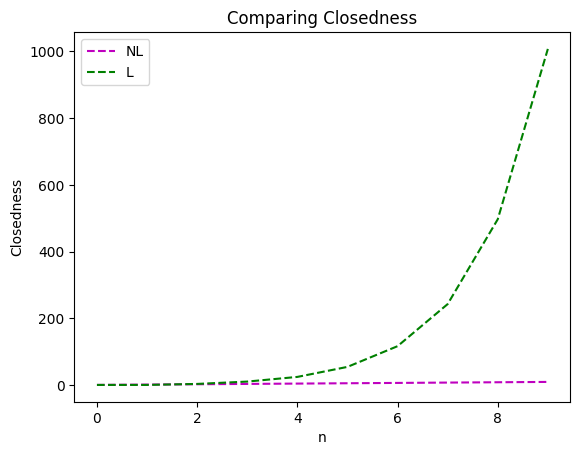
\includegraphics[width=\textwidth]{../statistics/plots/wrostDFA/Closedness.png}
    \caption{Closedness Problem Number}
    \label{fig:ClosednessWrostDFACompare}
  \end{subfigure}
  \begin{subfigure}[b]{0.3\textwidth}
    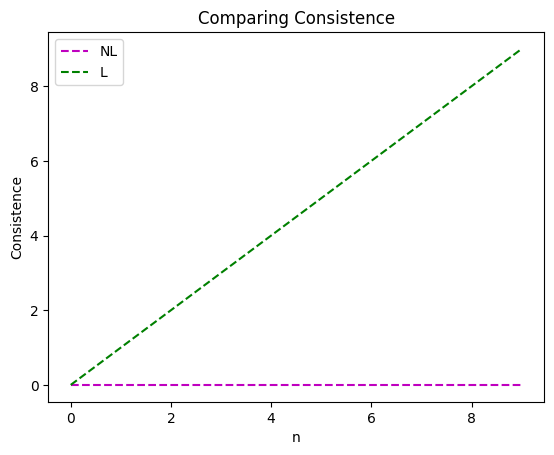
\includegraphics[width=\textwidth]{../statistics/plots/wrostDFA/Consistence.png}
    \caption{Consistence Problem Number}
    \label{fig:ConsistenceWrostDFACompare}
  \end{subfigure}
  % \begin{subfigure}[b]{0.3\textwidth}
  %   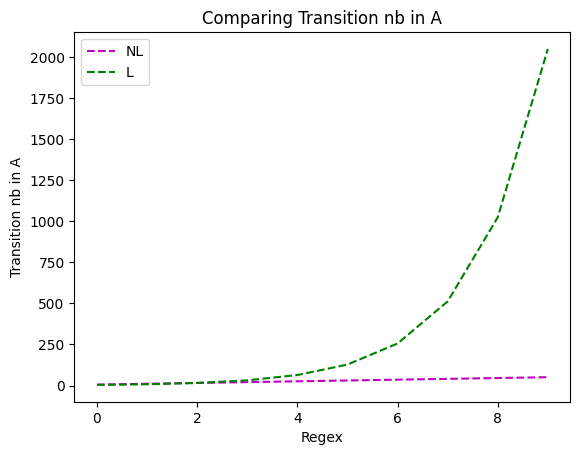
\includegraphics[width=\textwidth]{../statistics/plots/wrostDFA/Transition nb in A.png}
  %   \caption{Transition Number}
  %   \label{fig:TransitionWrostDFACompare}
  % \end{subfigure}
  \caption{mDFA vs cRFSA on $U = regex((a+b)^*a(a+b)^n)$}
  \label{fig:wrostDFA}
\end{figure}

From \cref{fig:wrostDFA}, we can see that the \textit{L*} is much more excpensive thant \textit{NL*} we can see that as announced the number of states of the \textit{mDFA} is exponentially bigger then the \textit{cRFSA} but we can also see how the number of states really impcat the number of membership queries and the number of times the table is found to be not closed.

However we can also note that interestingly the number of equivalence queries is the same for the two algorithms since in fact if $n = 0$ the algorithms understand the language after only one equivalence query, after the first three three membership queries the table is learned and if $n > 1$ only two equivalence queries are sufficient beacuase the first is sent as for the previous case after the first three membership queries. Then the \textit{Teacher} provides the counter-example which is enough to distinguish every new residual until the \textit{Observation Table} becomes closed and consistent and this time the second conjecture perfefctly recognizes $U$.

An other particular phenomen we can see is the number of time the table is found not consistent, which grows linearly for the \textit{L*} instead of being exponentially as for the two other plots.

Let's suppose that we are the \textit{Learner} then we send our first three membership queries we think that the language is the empty one since $\forall x \in{\varepsilon, a, b}, \text{ the Teacher answers that } x \notin U$. The first counter-exemple we receive is the shortest word belonging to $U$ which in this case is a word $w$ of length $n+1$ with a leading $a$ where $w \in U \text{ and } \forall x \in Pref(w) | x \neq w \rightarrow x \notin U$. Futhermore, for every prefix x and y different from w, x and y belong to two different residuals and all of them are exactly the prime residuals of $U$. From these prime residual \textit{L*} is capable to reconstruct the composed residual while adding column in $E$. On the other hand \textit{NL*} since it adds the first counter-exemple in $E$ it is able to find prime without having any consistence problem, since every new row will be prime and so the verification of closedness is enough to understand the language.

\subsubsection{Size(RFSA) is exponentially bigger than Size(mNFA)}
In this section we are going to show the behaviour of the two algorithms on a particular class of regular expressions depending on a fixed parameter $n$ where \textit{cRFSA} has exactly the same size of the \textit{mDFA} but where the corresponding \textit{mNFA} is exponentially smaller.\\
This automaton is built recursively and is proposed in Section 6 of \cite{RFSA}. The construction is done for an automaton $A_n = \langle \Sigma, Q, Q_I, F, \delta \rangle $ where :
\begin{itemize}
  \item $\Sigma = {a, b}$,
  \item $Q = \{q_i | 0 \leq i < n-1 \}$,
  \item $Q_I = \{q_i | 0 \leq i < n/2\}$,
  \item $F = q_0$
  \item $\delta(q_i,a) = q_i+1$for $0 \leq i< n - 1$, $\delta(q_{n-1},a) = q_0$, $\delta(q_0,b)=q_0$, $\delta(q_i,b) = q_{i-1}$ for $1<i<n$ and $\delta(q_1,b)=q_{n-1}$.
\end{itemize}

As proved in that paper, the number of state a \textit{mNFA} equals the parameter $n$ of the automaton, but the number of states of the \textit{cRFSA} is exponential with reference to $n$.\\
The statistics of the execution of the two algorithms are shown in \cref{fig:wrostRFSA}.

\begin{figure}[!htb]
  \centering
  \begin{subfigure}[b]{0.3\textwidth}
    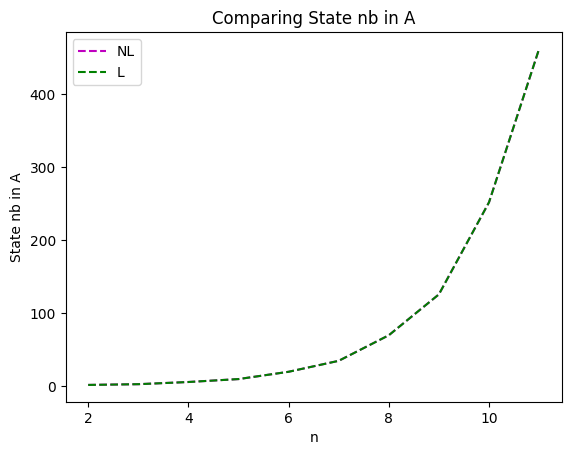
\includegraphics[width=\textwidth]{../statistics/plots/wrostRFSA/State nb in A.png}
    \caption{Comparing State Number}
    \label{fig:StateWrostRFSACompare}
  \end{subfigure}
  \begin{subfigure}[b]{0.3\textwidth}
    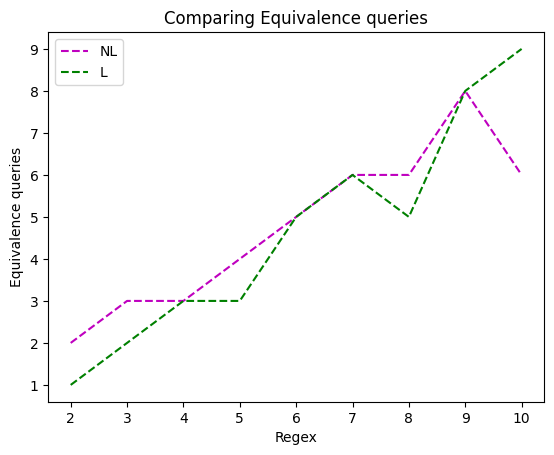
\includegraphics[width=\textwidth]{../statistics/plots/wrostRFSA/Equivalence queries.png}
    \caption{Equivalence queries Number}
    \label{fig:EquivWrostRFSACompare}
  \end{subfigure}
  \begin{subfigure}[b]{0.3\textwidth}
    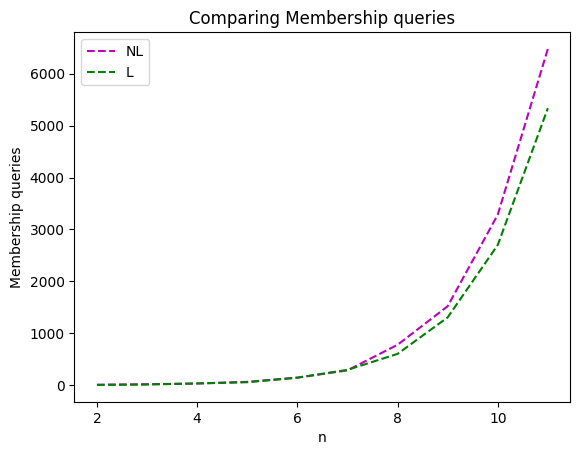
\includegraphics[width=\textwidth]{../statistics/plots/wrostRFSA/Membership queries.png}
    \caption{Membership queries Number}
    \label{fig:MemberWrostRFSACompare}
  \end{subfigure}
  \begin{subfigure}[b]{0.3\textwidth}
    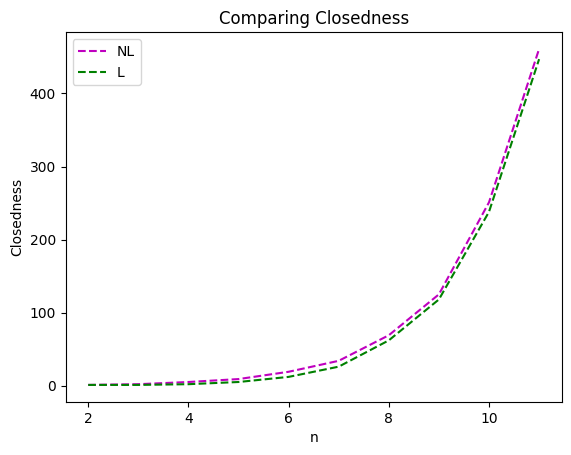
\includegraphics[width=\textwidth]{../statistics/plots/wrostRFSA/Closedness.png}
    \caption{Closedness Problem Number}
    \label{fig:ClosednessWrostRFSACompare}
  \end{subfigure}
  \begin{subfigure}[b]{0.3\textwidth}
    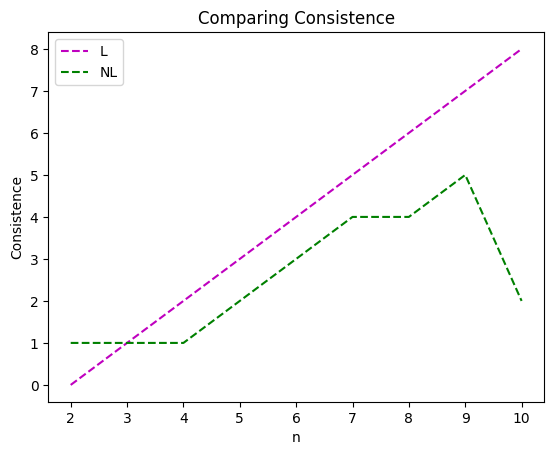
\includegraphics[width=\textwidth]{../statistics/plots/wrostRFSA/Consistence.png}
    \caption{Consistence Problem Number}
    \label{fig:ConsistenceWrostRFSACompare}
  \end{subfigure}
  % \begin{subfigure}[b]{0.3\textwidth}
  %   \includegraphics[width=\textwidth]{../statistics/plots/wrostRFSA/Transition nb in A.png}
  %   \caption{Transition Number}
  %   \label{fig:TransitionWrostRFSACompare}
  % \end{subfigure}
  \caption{mDFA vs cRFSA on $U = L(A_n)$}
  \label{fig:wrostRFSA}
\end{figure}

We can see that the number of state are the same for the two class of Automata and that the number of Membership an Closedness problems are similar. What change is the number of equivalence queries which is particularly smaller for the \textit{NL*} algorithm as for the number of time where the \textit{O.T.} is found not consistent. This is because adding counter-exemples in $E$ instead of $S$ is in general a good mean to be able to distinguish autonomously newer residuals. New residuals are also useful to reduce the number of Consistence problem increasing however the number of Closedness problem.

\subsection{Results over generical Teachers}

The third type of comparaison has been performed over a huge number of \textit{Teachers} on the form of automaton of size varying from $1$ to $100$. In this way we are able to see in averege the performances of \textit{L} versus \textit{NL*}.

This benchmark has been done taking the \textit{Automata} from the \textit{GitHub} repository \url{https://github.com/parof/buchi-automata-benchmark}. Every automaton is supposed to represent a \textit{Büchi Automaton} and I have reused them to create \textit{mDFA}: after determinization and minimisation, I was able to get a lot of different \textit{mDFA} which I have sorted by number of states. Every \textit{Automaton} of the list has been transformed into a \textit{Teacher} and then, one by one, every \textit{Teacher} has been submitted to \textit{L*} and \textit{NL*} to get at the end the same statistics as before.

\begin{figure}[!htb]
  \centering
  \begin{subfigure}[b]{0.3\textwidth}
    \includegraphics[width=\textwidth]{../statistics/plots/BenchMark/State nb in A.png}
    \caption{Comparing State Number}
    \label{fig:StateBenchMarkCompare}
  \end{subfigure}
  \begin{subfigure}[b]{0.3\textwidth}
    \includegraphics[width=\textwidth]{../statistics/plots/BenchMark/Equivalence queries.png}
    \caption{Equivalence queries Number}
    \label{fig:EquivBenchMarkCompare}
  \end{subfigure}
  \begin{subfigure}[b]{0.3\textwidth}
    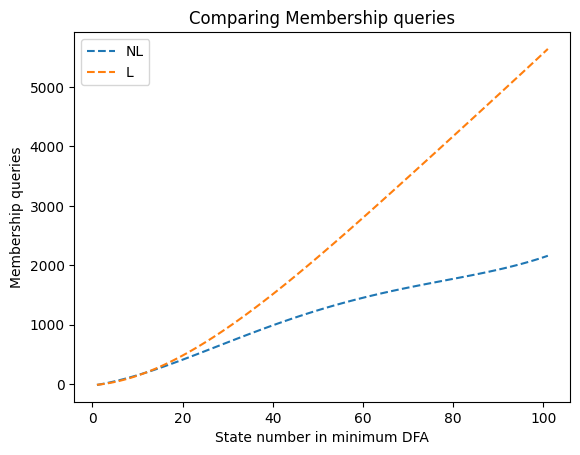
\includegraphics[width=\textwidth]{../statistics/plots/BenchMark/Membership queries.png}
    \caption{Membership queries Number}
    \label{fig:MemberBenchMarkCompare}
  \end{subfigure}
  \begin{subfigure}[b]{0.3\textwidth}
    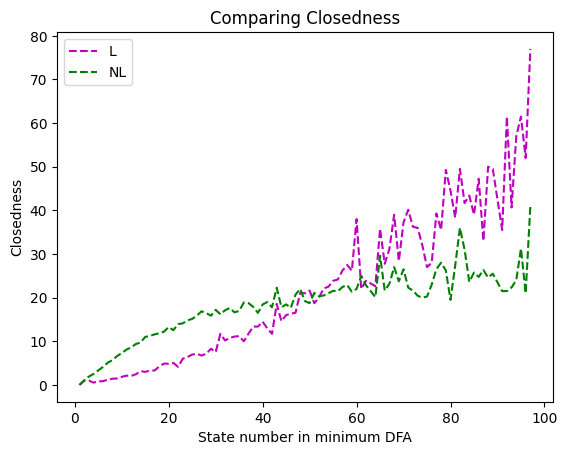
\includegraphics[width=\textwidth]{../statistics/plots/BenchMark/Closedness.png}
    \caption{Closedness Problem Number}
    \label{fig:ClosednessBenchMarkCompare}
  \end{subfigure}
  \begin{subfigure}[b]{0.3\textwidth}
    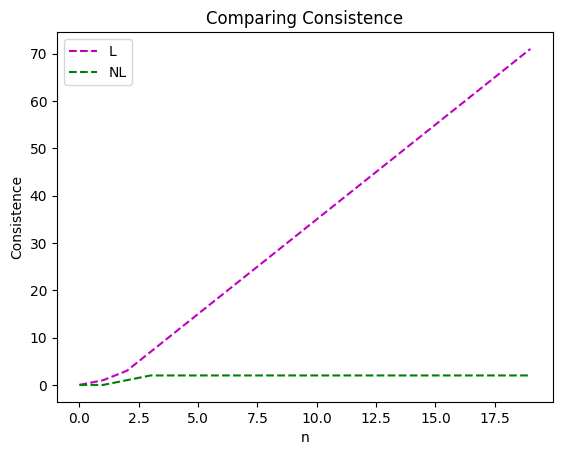
\includegraphics[width=\textwidth]{../statistics/plots/BenchMark/Consistence.png}
    \caption{Consistence Problem Number}
    \label{fig:ConsistenceBenchMarkCompare}
  \end{subfigure}
  \begin{subfigure}[b]{0.3\textwidth}
    \includegraphics[width=\textwidth]{../statistics/plots/BenchMark/Transition nb in A.png}
    \caption{Transition Number}
    \label{fig:TransitionBenchMarkCompare}
  \end{subfigure}
  \caption{mDFA vs cRFSA on random Teachers}
  \label{fig:benchmark}
\end{figure}

We see in \cref{fig:benchmark} that as expected the number of state of \textit{cRFSA} is in general exponentially smaller than the \textit{mDFA} and that the number of equivalence and membership queries is about everitime the \textit{NL*} algorithm that outperform \textit{L*}. As expected the number of Consistence problem is won by the \textit{NL*} but curiously the Closedness comparaison is taken by the \textit{NL*} only after about $50$ states. We can intuitively understand that before $50$ states the \textit{Automata} generated by \textit{L*} and \textit{NL*} are in general pretty similar and so it is clear that adding every counter-exemple in $E$ cause the \textit{NL*} algorithm to find a lot of time the table to be not Close. In \cref{fig:TransitionBenchMarkCompare} we see that the number of transisitions of the \textit{mDFA} is linear to the number of its states, whereas the number of transisitions in the \textit{cRFSA}, even if it's number of states is exponentially smaller in averege then the \textit{mDFA}, is clearly bigger then the \textit{mDFA}. This is due to the fact that the \textit{cRFSA} tend to create a transition from a state $q_i$ to every state $q_i'$ if $L(q_i') \sqsubseteq L(q_i)$.

\section{Conclusion}

In this paper, we have seen some idea on how regular languages can be understood in different way. We can build finite state automata which can be deterministic and so easy to understand by humans but which can take a lot of space in memory or non-deterministic automata which are less intuitive expacially if these automata have a lot of transition but which can be exponentially smaller than a \textit{mDFA}.

Other studies have been done to seek other way to create automaton which can be smaller then \textit{cRFSA}, for exemple we can have automata that uses logical operators on transitions such as the \textit{Alternating Finite State Automata} or other automata using symbolique links between symbols of the alphabet.

All of these algorithms are all an evolution of the \cite{LPaper} but works only on languages which are regular. It should be interesting to see if we are able to develop this concept of learning algorithms to languages belonging to grammars which my be context free, context sensitive and so on. But it is clear that the less limitation we add in our langauge, the more complicate will be to understand it.

\subsection{Thanks}
I would like to thanks Mme Di Giusto and Mr Lozes for their support during the development of this study, they have been really helpful to suggest me differnt approches to analyse and different point of view to interpretate the results I obtained.